A different way of encoding spikes is using a \emph{rank-order}; this means
keep just the order in which those spikes were fired and disregard the exact timing. One can think of this as a compromise between the complexity of time-based encoding and the small capacity to represent information of rate-based codes. Rank-ordered spike trains have been used in vision tasks under a biological plausibility constraint, making them a viable way of image encoding for neural applications~[\cite{van-rullen-rate-coding,basab-model}].

We perform rank-ordered encoding using an algorithm known as 
\emph{FoCal}~[\cite{basab-model}]. It models the \emph{foveal pit} region, the highest resolution area of the retina. As a first step, four discrete 2D \emph{convolutions} are performed. Each convolution simulates a ganglion cell type and every cell is modelled using Differences of Gaussians (DoG, Eq.~\ref{eq-dog}). 
\begin{equation}
\label{eq-dog}
DoG_w(x,y) = \pm\frac{1}{2\pi\sigma_{w,c}^2}e^{\frac{-(x^2 + y^2)}{2\sigma_{w,c}^2}}
\mp\frac{1}{2\pi\sigma_{w,s}^2}e^{\frac{-(x^2 + y^2)}{2\sigma_{w,s}^2}}
\end{equation}
where $\sigma_{w,c}$ and $\sigma_{w,s}$ are the standard deviation for the 
centre and surround components of the DoG at scale $w$ (cell type). The signs 
will be ($-$,$+$) if the ganglion cell has an \emph{off-centre} behaviour and 
($+$,$-$) if it has an \emph{on-centre} one. Table~\ref{tab-kernel-specs} 
describes the parameters used to compute the convolution \emph{kernels} at each 
scale $w$.

\begin{table}[htb]
  \caption{Simulation parameters for ganglion cells}
  \centering
  \begin{tabular}{l c c c c}
    \begin{minipage}{1.2cm}Cell type \end{minipage}& 
    \begin{minipage}{1cm} \centering Matrix width \end{minipage}&  
    \begin{minipage}{1.3cm}\centering Centre std. dev. ($\sigma_c$)\vspace*{0.1cm}\end{minipage} & 
    \begin{minipage}{1.3cm}\centering Surround std. dev. ($\sigma_s$)\vspace*{0.1cm}\end{minipage} & 
    \begin{minipage}{1.3cm}\centering Sampling resolution (cols,rows)\vspace*{0.1cm}\end{minipage} \\
    \hline
    \begin{minipage}{1.32cm}\vspace*{0.1cm} Midget Off-centre \vspace*{0.005cm} \end{minipage}& 
    \begin{minipage}{1cm}\centering$3$ \end{minipage}& 
    $0.8$ & $6.7 \times \sigma_c$ &  1, 1 \\
    \begin{minipage}{1.32cm} Midget On-centre \vspace*{0.005cm}\end{minipage} & 
    \begin{minipage}{1cm}\centering $11$ \end{minipage}& 
    $1.04$ & $6.7 \times \sigma_c$ & 1, 1 \\
    \begin{minipage}{1.32cm}Parasol Off-centre \vspace*{0.005cm}\end{minipage} & 
    \begin{minipage}{1cm}\centering $61$ \end{minipage}& 
    $8$ & $4.8 \times \sigma_c$ & 5, 3 \\
    \begin{minipage}{1.32cm} Parasol On-centre \vspace*{0.005cm}\end{minipage} & 
    \begin{minipage}{1cm}\centering $243$\end{minipage} &
    $10.4$ & $4.8 \times \sigma_c$ & 5, 3 
  \end{tabular}
  \label{tab-kernel-specs}
\end{table}

Every pixel value in the convolved images (Fig. \ref{fig-convolution-results}) 
is inversely proportional to a spike emission time (i.e. the higher the pixel value, the sooner the spike will be sent out.)

\begin{figure}[hbt]
  \centering
  \subfloat[Original image]{
    \label{sfig-rank-ordered-original}
    
\includegraphics[width=0.15\textwidth]{original_5_1}
  }
  \subfloat[Midget Off-centre]{
    \label{sfig-rank-ordered-midget-off}
    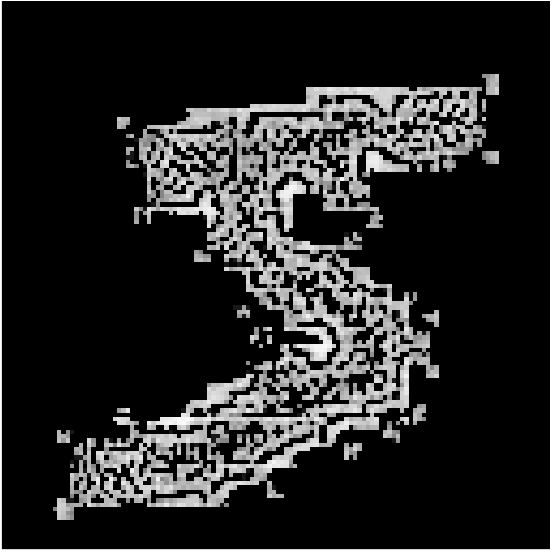
\includegraphics[width=0.15\textwidth]{filtered_focal_5_1_0}
  }
  \subfloat[Midget On-centre]{
    \label{sfig-rank-ordered-midget-on}
    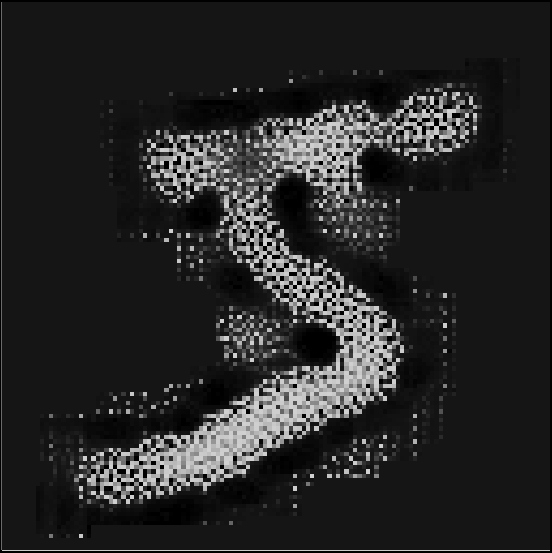
\includegraphics[width=0.15\textwidth]{filtered_focal_5_1_1}
  }\\
  \subfloat[Parasol Off-centre]{
    \label{pic-lena-P-OFF}
    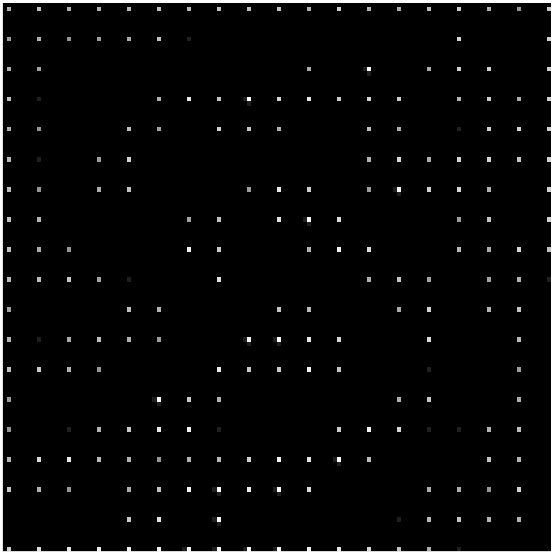
\includegraphics[width=0.15\textwidth]{filtered_focal_5_1_2}
  }
  \subfloat[Parasol On-centre]{
    \label{pic-lena-P-ON}
    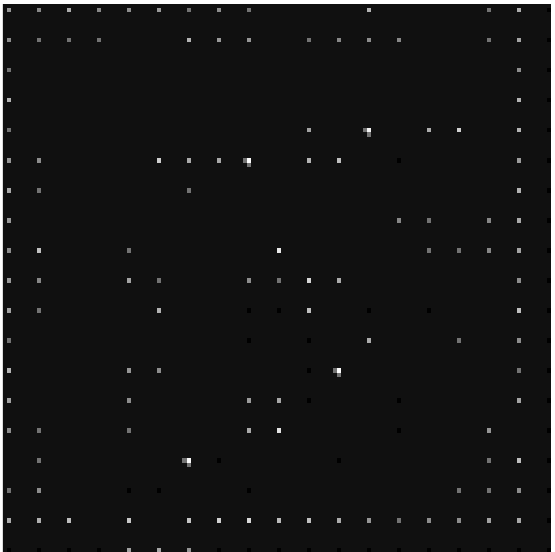
\includegraphics[width=0.15\textwidth]{filtered_focal_5_1_3}
  }
  \caption{Results of simulating ganglion cells (convolved images are enhanced for better contrast)}
  \label{fig-convolution-results}
\end{figure}
The algorithm also performs redundancy a correction step; it does so by 
adjusting the convolved image's pixel value according to the correlation 
between convolution kernels. At each iteration of the correction step, the 
maximum coefficient value of \emph{all images} is selected, ``taken out'' and its surrounding pixels get adjusted (Alg.~\ref{code-focal-corr}).
\begin{algorithm}[h]
  \caption{FoCal, Part 2}
  \label{code-focal-corr}
  \begin{algorithmic}
    \Procedure{Correction}{coeffs $C$, correlations $Q$}
    \State $N \leftarrow \emptyset$ \Comment{Corrected coefficients}
    \Repeat
    \State $m \leftarrow max(C)$\Comment{Obtain maximum from $C$}
    \State $M \leftarrow M \cup m$\Comment{Add maximum to $M$}
    \State $C \leftarrow C \setminus m$\Comment{Remove maximum from $C$}
    \ForAll{$ c \in C$} \Comment{Adjust all remaining $c$}
    \If{$Q(m, c) \neq 0$} \Comment{Adjust only near}
    \State $c \leftarrow c - m \times Q(m, c)$
    \EndIf
    \EndFor
    \Until{$C = \emptyset$}
    \State \textbf{return} $M$
    \EndProcedure
  \end{algorithmic}
\end{algorithm}
Two resolutions are provided for the rank-order encoded database, the first is 
the original $28\times28$ one. An additional up-scaled resolution version is also provided, the images where scaled to a $128\times128$ resolution using bi-cubic interpolation, this was done to match the DVS native resolution. The format of the data is not exactly AER since keeping spiking order is what matters for this encoding; depending
on the experimenter's needs the timing between spikes can be modified. The adjusted weights and cell origin have been preserved for further processing.